%%
%% This is file `sample-manuscript.tex',
%% generated with the docstrip utility.
%%
%% The original source files were:
%%
%% samples.dtx  (with options: `manuscript')
%% 
%% IMPORTANT NOTICE:
%% 
%% For the copyright see the source file.
%% 
%% Any modified versions of this file must be renamed
%% with new filenames distinct from sample-manuscript.tex.
%% 
%% For distribution of the original source see the terms
%% for copying and modification in the file samples. dtx.
%% 
%% This generated file may be distributed as long as the
%% original source files, as listed above, are part of the
%% same distribution. (The sources need not necessarily be
%% in the same archive or directory.)
%%
%% The first command in your LaTeX source must be the \documentclass command.
%%%% Small single-column format, used for CIE, CSUR, DTRAP, JACM, JDIQ, JEA, JERIC, JETC, PACMCGIT, TAAS, TACCESS, TACO, TALG, TALLIP (formerly TALIP), TCPS, TDSCI, TEAC, TECS, TELO, THRI, TIIS, TIOT, TISSEC, TIST, TKDD, TMIS, TOCE, TOCHI, TOCL, TOCS, TOCT, TODAES, TODS, TOIS, TOIT, TOMACS, TOMM (formerly TOMCCAP), TOMPECS, TOMS, TOPC, TOPLAS, TOPS, TOS, TOSEM, TOSN, TQC, TRETS, TSAS, TSC, TSLP, TWEB.
% \documentclass[acmsmall]{acmart}

%%%% Large single-column format, used for IMWUT, JOCCH, PACMPL, POMACS, TAP, PACMHCI
% \documentclass[acmlarge,screen]{acmart}

%%%% Large double-column format, used for TOG
% \documentclass[acmtog, authorversion]{acmart}

%%%% Generic manuscript mode, required for submission
%%%% and peer review
%\documentclass[manuscript,screen,review]{acmart}
\documentclass[sigconf,review]{acmart}


%% Fonts used in the template cannot be substituted; the margin 
%% adjustments are not allowed.
%%
%% \BibTeX command to typeset the BibTeX logo in the docs
\AtBeginDocument{%
 \providecommand\BibTeX{{%
   \normalfont B\kern-0.5em{\scshape i\kern-0.25em b}\kern-0.8em\TeX}}}
    
  %  \AtBeginDocument{\renewcommand*{\thesubfigure}{\alphalph{\value{subfigure}}}}

%% Rights management information.  This information is sent to you
%% when you complete the rights form.  These commands have a SAMPLE
%% values in them; it is your responsibility as an author to replace
%% the commands and values with those provided to you when you
%% complete the rights form.


\setcopyright{none} % remove permission section
\settopmatter{printacmref=false} % remove ACM reference format
\renewcommand\footnotetextcopyrightpermission[1]{} % removes footnote with conference information in the first column
\pagestyle{plain}
%\setcopyright{acmcopyright}
%\copyrightyear{2022}
%\acmYear{2022}
%\acmDOI{00.0000/0000000.0000000}

%% These commands are for a PROCEEDINGS abstract or paper.
%\acmConference[Woodstock '18]{Woodstock '18: ACM Symposium on Neural Gaze Detection}{June 03--05, 2018}{Woodstock, NY}
  \acmConference[MSR 2022]{MSR '22: Proceedings of the 19th International Conference on Mining Software Repositories}{May 23–24, 2022}{Pittsburgh, PA, USA}
\acmBooktitle{MSR '22: Proceedings of the 19th International Conference on Mining Software Repositories, May 23–24, 2022, Pittsburgh, PA, USA}
\acmPrice{15.00}
\acmISBN{978-1-4503-XXXX-X/18/06}

\newcommand{\instructor}[1]{\textcolor{blue}{{\it [Instructor: #1]}}}
\usepackage{xspace}
\newcommand{\ie}{\textit{i.e.}}
\newcommand{\eg}{\textit{e.g.}}
\newcommand{\etal}{\textit{et al. \xspace}}
%\usepackage{array}
%\newcolumntype{L}{>{\arraybackslash}m{8cm}}
%%%%% Long text wrap %%%%%
\usepackage{array}
\newcolumntype{L}{>{\arraybackslash}m{16cm}}
%\newcolumntype{L}[1]{>{\raggedright\let\newline\\arraybackslash\hspace{0pt}}m{#1}}
\newcolumntype{C}[1]{>{\centering\let\newline\\arraybackslash\hspace{0pt}}m{#1}}
\newcolumntype{R}[1]{>{\raggedleft\let\newline\\arraybackslash\hspace{0pt}}m{#1}}
%%%%% Long text wrap %%%%%
%\usepackage{adjustbox}
%\usepackage{subcaption}
%\usepackage{textcomp}
%\usepackage{pgfplots}
\usepackage[numbered]{bookmark}
%\usepackage{soul}
%\usepackage{booktabs}
%\usepackage{multirow}
%\usepackage{float}
%\usepackage{url}
\usepackage{tcolorbox}
\usepackage{graphicx}
%\usepackage{textcomp}
\usepackage{xcolor}
%\usepackage{url}
%\usepackage{tabularx} 
%\usepackage{balance}
\usepackage{stfloats}
\usepackage{fullpage}
\usepackage[justification=centering]{caption}
\usepackage{lineno}
\usepackage[title]{appendix}
\usepackage{dirtytalk}
\usepackage{amsmath}
%\usepackage{tikz}
\usepackage{pgfplots, pgfplotstable}
%\usetikzlibrary{tikzmark}
\usetikzlibrary{patterns}



%%%%%
%-----------------------
%\usepackage[utf8]{inputenc}
\usepackage[english]{babel}
%\usepackage{amssymb}
\usepackage{textcomp}
%\usepackage{indentfirst}
%\setcounter{tocdepth}{3}
\usepackage{mathtools}
%\usepackage[usestackEOL]{stackengine}
%\usepackage{amsmath}
\usepackage{ltxtable}
\usepackage{algorithm}
\usepackage{algpseudocode}
\usepackage{textcomp}
%\usepackage{mathpazo}
%\usepackage{tgpagella}
%-----------------------

\usepackage{tcolorbox}

%\usepackage[dvipsnames]{xcolor}
\usepackage{pgf-pie}
%\usepackage{pgfplots}
%\pgfplotsset{compat=1.14}
%%%%%%%%%%%%%%%%%%%%%%%%%%%%%%%%%%%%%%%%%%%%%%%%%%%
\definecolor{wedge1}{RGB}{ 190  30  46}
\definecolor{wedge2}{RGB}{ 240  65  54}
\definecolor{wedge3}{RGB}{ 241  90  43}
\definecolor{wedge4}{RGB}{ 247 148  30}
\definecolor{wedge5}{RGB}{  43  56 144}
\definecolor{wedge6}{RGB}{  28 117 188}
\definecolor{wedge7}{RGB}{  40 170 225}
\definecolor{wedge8}{RGB}{ 119 179 225}
\definecolor{wedge9}{RGB}{ 181 212 239}
\definecolor{wedge10}{RGB}{  0 104  56}
\definecolor{wedge11}{RGB}{  0 148  69}
\definecolor{wedge12}{RGB}{ 57 181  74}
\definecolor{wedge13}{RGB}{141 199  63}
\definecolor{wedge14}{RGB}{215 244  34}
\definecolor{wedge15}{RGB}{249 237  50}
\definecolor{wedge16}{RGB}{248 241 148}
\definecolor{wedge17}{RGB}{242 245 205}
\definecolor{wedge18}{RGB}{123  82  49}
\definecolor{wedge19}{RGB}{104  73 158}
\definecolor{wedge20}{RGB}{102  45 145}
\definecolor{wedge21}{RGB}{148 149 151}
\definecolor{wedge22}{RGB}{ 204 50 153}
\definecolor{wedge23}{RGB}{ 79 47 79}
\definecolor{wedge24}{RGB}{ 173 234 234}
\definecolor{wedge25}{RGB}{ 216 191 216}
\definecolor{wedge26}{RGB}{  43  56 144}
\definecolor{wedge27}{RGB}{  40 170 225}
\definecolor{wedge28}{RGB}{ 119 179 225}
\definecolor{wedge29}{RGB}{ 181 212 239}
\definecolor{wedge30}{RGB}{  0 104  56}
\definecolor{wedge31}{RGB}{  0 148  69}
\definecolor{wedge32}{RGB}{ 57 181  74}

\usetikzlibrary{chains}
%%%%%%%%%%%%%%%%%%%%%%%%%%%%%%%%%%%%%%


\def\groupTotals{{1,4,5,8,1,2}}
\pgfmathsetmacro\startAngle{90-3.6/2}
\pgfmathsetmacro\radius{+5}
\pgfmathsetmacro\maxLeg{+12}
\pgfmathsetmacro\legBound{+60}
\pgfmathsetmacro\legSpacing{2*\legBound/(\maxLeg-1)}
%%%%%%%%%%%%%%%%%%%%%%%%%%%%%%%%%%%%%%

%%%%%%%%%%%%%%%%%%%%%%%%%%%%%%%%%%%%%
\usepackage{verbatim}
%\usepackage{pgfplots, pgfplotstable}
%\pgfplotsset{width=7cm,compat=1.8}
%\pgfplotsset{width=7cm,compat=1.8,tick label style={font=\small}}
\pgfplotsset{compat=1.14}
\usetikzlibrary{patterns,}

\usepackage{graphicx}
\usepackage{tabularx,booktabs}
\usepackage{array}
\usepackage{bbding}
\usepackage{pifont}
\usepackage{wasysym}
%\usepackage{amssymb}
\usepackage{caption}
\usepackage{dirtytalk}
%\usepackage[showframe]{geometry}
%\usepackage{subfigure}
\usepackage{subcaption}
%\usepackage{amsmath} % Star
%\usepackage[table]{xcolor}
\usepackage{tabularx}
%\usepackage{pgfplots}
%\usepackage{pgf-pie}
%\usepackage{verbatim}
%\usepackage{pgfplotstable}
\usepackage{sfmath}
\usepackage{array, booktabs, makecell}
\usepackage{color}
%\usepackage[dvipsnames]{xcolor}
\usepackage{csquotes}
\usepackage{url}
\usepackage{comment}
\usepackage{tikz}
\usepackage{balance}
\usepackage{listings}
\usepackage{booktabs} % used for \toprule in tables
%\usepackage{cite}
\usepackage{soul} % highlighting
\urlstyle{same} %% footnote fonts
\usetikzlibrary{fit} %% Used for putting the dotted box in the image
%\usepackage[margin=2cm]{geometry}
\usetikzlibrary{positioning}
\usetikzlibrary{arrows}
\usetikzlibrary{shapes.multipart}
%\usepackage{caption}
%\usepackage{graphicx}
\usepackage{adjustbox}
%\usepackage{tablefootnote}
\usepackage{float}
\usepackage{rotating}
\usepackage{nth}
\DeclareCaptionType{TextBox}
\usepackage{pstricks}
%%%%%%%%%%%%%%%%%%%%%%%%%%%%%%%%%%%%%%%%%%%%%%%%%%%%%%%%
\usepackage{placeins}
\usepackage{afterpage}
\usepackage{multirow} 
\usepackage{textcomp}
\usepackage{multicol}
\usepackage{varwidth} % Double column tables

%%%%%

%\usepackage{subfigure}
\newcommand{\eman}[1]{\textcolor{violet}{{\it [Eman says: #1]}}}



%%
%% Submission ID.
%% Use this when submitting an article to a sponsored event. You'll
%% receive a unique submission ID from the organizers
%% of the event and this ID should be used as the parameter to this command.
%%\acmSubmissionID{123-A56-BU3}

%%
%% The majority of ACM publications use numbered citations and
%% references.  The command \citestyle{authoryear} switches to the
%% "author year" style.
%%
%% If you are preparing content for an event
%% sponsored by ACM SIGGRAPH, you must use the "author year" style of
%% citations and references.
%% Uncommenting
%% The next command will enable that style.
%%\citestyle{acmauthoryear}

%%
%% end of the preamble, the start of the body of the document source.
\begin{document}

%%
%% The "title" command has an optional parameter,
%% allowing the author to define a "short title" to be used in page headers.
\title{Test Smells for Flaky Test Prediction}


\author{Pranay Reddy Juturu}
%\authornote{Both authors contributed equally to this research.}
\email{pjuturu@stevens.edu}
\affiliation{%
  \institution{Stevens Institute of Technology}
  %\streetaddress{P.O. Box 1212}
  \city{Hoboken}
  \state{New Jersey}
  \country{USA}
  %\postcode{43017-6221}
}

\author{Ashay Pable}
%\authornote{Both authors contributed equally to this research.}
\email{apable@stevens.edu}
\affiliation{%
  \institution{Stevens Institute of Technology}
  %\streetaddress{P.O. Box 1212}
  \city{Hoboken}
  \state{New Jersey}
  \country{USA}}
  
\author{Diya Sanghvi}
%\authornote{Both authors contributed equally to this research.}
\email{dsanghv1@stevens.edu}
\affiliation{%
  \institution{Stevens Institute of Technology}
  %\streetaddress{P.O. Box 1212}
  \city{Hoboken}
  \state{New Jersey}
  \country{USA}}
  

%%
%% The "author" command and its associated commands are used to define
%% the authors and their affiliations.
%% Of note is the shared affiliation of the first two authors and the
%% "authornote" and "authornotemark" commands
%% used to denote shared contribution to the research.


%%
%% By default, the full list of authors will be used on the page
%% headers. Often, this list is too long and will overlap
%% other information printed in the page headers. This command allows
%% the author to define a more concise list
%% of authors' names for this purpose.
%\renewcommand{\shortauthors}{Trovato and Tobin, et al.}

%%
%% The abstract is a short summary of the work to be presented in the
%% article.
\begin{abstract}
Flaky tests are tests that provide variable results even when run under identical conditions. These tests can be a blocker to the development process since they produce false-positive and false-negative results and increase testing time and cost. To ensure the reliability and correctness of the software testing process, flaky tests must be identified and eliminated. Test smells, on the other hand, signal possible problems with the test code, such as bad design or a lack of maintenance. Researchers have been investigating the use of test smells as a sign of flaky tests in recent years, as they may identify underlying flaws in the test code that can contribute to flakiness. We explore the various sorts of test smells that have been detected, as well as the methodologies used to identify them, as well as methods for predicting flaky tests using test smells. We also assess the efficacy of various approaches and identify gaps in current research that need to be addressed. Our approach emphasizes the potential of using test smells as an early warning system for flaky tests, as well as the need for additional research in this area to improve the accuracy and reliability of flaky test prediction.
\end{abstract}

%%
%% The code below is generated by the tool at http://dl.acm.org/ccs.cfm.
%% Please copy and paste the code instead of the example below.
%%
\begin{CCSXML}
<ccs2012>
 <concept>
  <concept_id>10010520.10010553.10010562</concept_id>
  <concept_desc>Computer systems organization~Embedded systems</concept_desc>
  <concept_significance>500</concept_significance>
 </concept>
 <concept>
  <concept_id>10010520.10010575.10010755</concept_id>
  <concept_desc>Computer systems organization~Redundancy</concept_desc>
  <concept_significance>300</concept_significance>
 </concept>
 <concept>
  <concept_id>10010520.10010553.10010554</concept_id>
  <concept_desc>Computer systems organization~Robotics</concept_desc>
  <concept_significance>100</concept_significance>
 </concept>
 <concept>
  <concept_id>10003033.10003083.10003095</concept_id>
  <concept_desc>Networks~Network reliability</concept_desc>
  <concept_significance>100</concept_significance>
 </concept>
</ccs2012>
\end{CCSXML}

\ccsdesc[500]{Software Engineering~AI for SE}
\ccsdesc[300]{Software Engineering}
%% \ccsdesc{Computer systems organization~Robotics}
%% \ccsdesc[100]{Networks~Network reliability}

%%
%% Keywords. The author(s) should pick words that accurately describe
%% the work being presented. Separate the keywords with commas.
\keywords{software quality, mining software repositories}

%% A "teaser" image appears between the author and the affiliation
%% information and the body of the document, and typically spans the
%% page.

%%
%% This command processes the author and affiliation and title
%% information and builds the first part of the formatted document.
\maketitle

\section{Introduction}
\label{Section:Introduction}
Binary classification is a vital activity in software development since it allows engineers to determine whether or not a program is showing a specific behavior. Regression testing is a crucial step in software development, as it helps to ensure that software is delivered continuously with quality and minimal failures after changes to the production code. During this phase, developers rely on the test results to determine whether a program has a bug resulting from recent changes. However, the presence of flaky tests can make this evaluation unreliable. Flaky tests are a type of test with an intermittent behavior that alternates between passing and failing when executed in the same codebase, without any changes. This non-deterministic behavior frustrates developers, as it makes it challenging to identify and fix the root cause of the problem. Additionally, flaky tests are difficult to debug and can cause delays in the release cycles, halting the development process.
Flaky tests can be a significant challenge in software development and identifying them is essential for ensuring the reliability and accuracy of test results. Dynamic and static approaches can be used to identify flaky tests, with each approach having its advantages and disadvantages.
Dynamic approaches involve re-executing test cases a fixed number of times, which can be expensive and error-prone. It can also be difficult to determine how many executions are enough to identify flakiness accurately. Static approaches, on the other hand, do not require code re-execution and rely on machine learning methods to predict flakiness likelihood based on various features obtained from the code.
Recently, an alternative approach for predicting flaky tests has been proposed based on identifying test smells. Test smells are associated with potential design problems in the test code, and their presence may impact software quality and lead to test flakiness. The alternative approach uses a set of predictors composed only of metrics collected statically, such as the size of the test case, the number of smells in the test code, and binary features related to the presence or absence of 19 test smells. The study found that this approach had better performance than the vocabulary-based model for cross-project prediction, achieving an F-measure of 0.83 with Random Forest.
We are extending the proposed solution by considering five new classifiers to predict the flaky tests. The inputs to the model will be the existence of test smells like assertion Roulette, and conditional Test Logic along with a list of some others (19 in total) with test flakiness as a boolean.
\\
 
\begin{itemize}
    \item Static approaches do not need the code to be executed again. Models built using static features have many advantages and are less costly.
    \item Pinto et al. \cite{r5}built a set of predictors considering that some patterns within the test code may be employed to identify flaky tests automatically.
    \item The authors came to the conclusion that the vocabulary-based strategy performs poorly when used across projects because it is context-sensitive and prone to overfitting.
    \item Considering this result, an alternative approach for flaky test prediction based on test smells is used. Test smells are associated with potential design problems in the test code.
    \item Test smells are a deviation from how tests should be created, arranged, and interacted with one another. That deviation can indicate issues with test design and negatively impact test performance.
    \item An open-source test smell detection tool, tsDetect is used. For each test case, this tool requires the identification of the corresponding production code to detect the test smells.
\end{itemize}



 \section{Related Work}
 \label{Section:RelatedWork}

We have come across some papers that compare various methods to predict flaky tests. First, 'An Evaluation of Machine Learning Methods for Predicting Flaky Tests'\cite{r1} utilizes Naive Bayes, Support Vector Machines (SVM), and Random Forests (RF) models and showed RF performed better when
it comes to precision (> 90\%) but provided very low recall (< 10\%) as compared to NB (i.e., precision < 70\% and recall >30\%). They extracted test cases from multiple open-source projects and used the dataset. Second, 'FlakeFlagger: Predicting Flakiness Without Rerunning Tests'\cite{r2} proposes a FlakeFlagger model that achieved a 60\% average precision on 24 Java projects while the highest being 90\% on spring-boot and going as low as 0\% on others. Other methods compared in the paper include the DeFlake model, a vocabulary-based approach, and a combined approach between the flake-flagger and a vocabulary-based approach that yielded the highest average precision of 66\%. One of the limitations in the paper appears to come from the fact that the authors had to supersample the data using SMOTE which some ML researchers are not very accepting of, Besides the 0\% accuracy clearly shows that the model may not be useful as a general algorithm. Third, 'DeFlaker: Automatically Detecting Flaky Tests'\cite{r3} introduces a software called deflaker, since this is an old paper, they do not use ML and try to use traditional software engineering techniques to solve the problem. However, they manage to achieve good accuracy on a given set of data, which might change if tested on a different dataset. They ran the software on 96 Java projects and claim to have a recall of 95\%. This high accuracy gave DeFlaker a place in the task and is used as a base software for comparison to many other papers like the one above mentioned. They utilize a lot of techniques and use the result to analyze and create a list of all flaky tests like AST builder, code coverage recorder, test outcome monitor, etc. All these techniques lead to pretty impressive results on their tested projects. However, such traditional processes may fail on a project out of their set and may not be general solutions to the problem at hand. Fourth, is our base paper 'On the use of test smells for prediction of flaky tests'\cite{r4}, which utilizes test smells for the prediction of flaky tests with the help of ML models like Random Forest, Decision Tree, KNN, LR, LDA, Perceptron, SVM, Naive Bayes, xgboost, bagging, stack, voting, NN. They claim to have achieved 83\% Precision and 83\% Recall on a Random Forest algorithm which was the highest they could achieve. Their dataset is extracted data from existing open-source projects.
  \begin{figure}
     \centering
     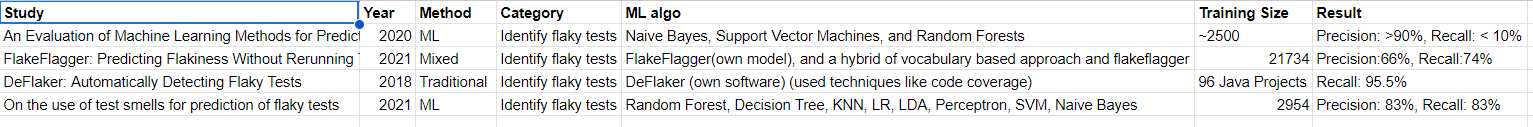
\includegraphics[width=8cm]{Screenshot 2023-04-10 205936.png}
     \caption{Related work review}
     \label{fig:relatedWork}
 \end{figure}
 

 \section{Study Design}
 \label{Section: Methodology} 
Our study aims to determine if test smells can be used to predict the existence of flaky tests. 

To find the test smells in the code, the authors employed a program called tsDetect\cite{r6}. Assertion roulette, conditional test logic, and mystery guest are just a few of the code patterns the program flags as being indicative of test smells. After that, the authors examined the test smells and took pertinent characteristics from the code. They used a feature selection technique known as mutual information to choose the most crucial attributes. The features with the highest mutual information score are chosen using this method, which assesses the dependencies between the features and the target variable (flaky tests). After feature selection, the authors used one-hot encoding to convert the data into a numerical format appropriate for machine learning techniques. We have considered five more classifiers XGBoost, Bagging, Stack, voting, and NN.
\\
The list of parameters as input to the model includes\cite{r6}:
\begin{itemize}
    \item Lines of code
    \item Smell Count
    \item Assertion Roulette
    \item Conditional Test Logic
    \item Constructor Initialization
    \item Default Test
    \item Duplicate Assert
    \item Eager Test
    \item Empty Test
    \item General Fixture
    \item Ignored Test
    \item Lazy Test
    \item Magic Number Test
    \item Mystery Guest
    \item Print Statement
    \item Redundant Assertion
    \item Resource Optimism
    \item Sensitive Equality
    \item Sleepy Test
    \item Unknown Test
    \item Verbose Test
\end{itemize}

After studying the data we decided to drop empty columns as well as rows that contain some empty entries for categorical columns because these empty entries do not provide any information to the model. To increase the dataset's quality and guarantee that we are only using pertinent data to train our models, empty columns and rows should be removed. The columns 'Author Email', 'Author Name', 'Committer Email', 'Committer Name', 'Commit Message', 'Commit SHA', 'file path', and 'Line' is removed. These columns either have no bearing on our goal or include categorical items with blank. Once this was done we decided to drop columns with zero relevance to the target column Klass which is Binary making it a binary classification. The columns that have zero relevance to the target columns are 'App', 'Build time in minutes', 'TimeStamp', and 'Version'. We have used random forest, decision trees, Naive Bayes, KNN, LDA, NN, voting, stack, bagging, xgboost, and Logistic Regression models. Grid search with cross-validation is used to adjust the hyperparameters for each model and the model with the best validation set performance is chosen. The random forest provides the best results out of the tested models. We use k-fold cross-validation, where we divide the data into k subsets and use each subset as a validation set in turn, to guarantee that our results are not overfitting the training data. This procedure is repeated k times, and the average performance over all iterations is reported. The evaluation metrics we used are Accuracy, Precision, Recall, F1 score, Matthews correlation coefficient, and Area Under the Curve.
The performance of each of the models is expressed and compared in the further sections of this paper. From studying the data we also concluded that the dataset only identifies if a test is flaky with a binary representation without the inclusion of any magnitude to provide the extent of flakiness, which might produce some limitations and could be scope for future experimentation.
For embedding of text inputs we are using CountVectorizer and TfidfVectorizer from the sklearn.feature\_extraction.text class.

Our dataset consists of data coming from a variety of famous GitHub projects and extracting information, like commit messages, analyzing tests, LOC, etc.

Our workflow will consist of information extraction from Github repositories, specifically the commit messages, and analyzing tests to identify test smells. This information is then used to feed data into our classifier once the text from the commit messages is tokenized and embedded. This is then fed into the trained model to classify the data point into flaky or not flaky.
 \begin{figure}
     \centering
     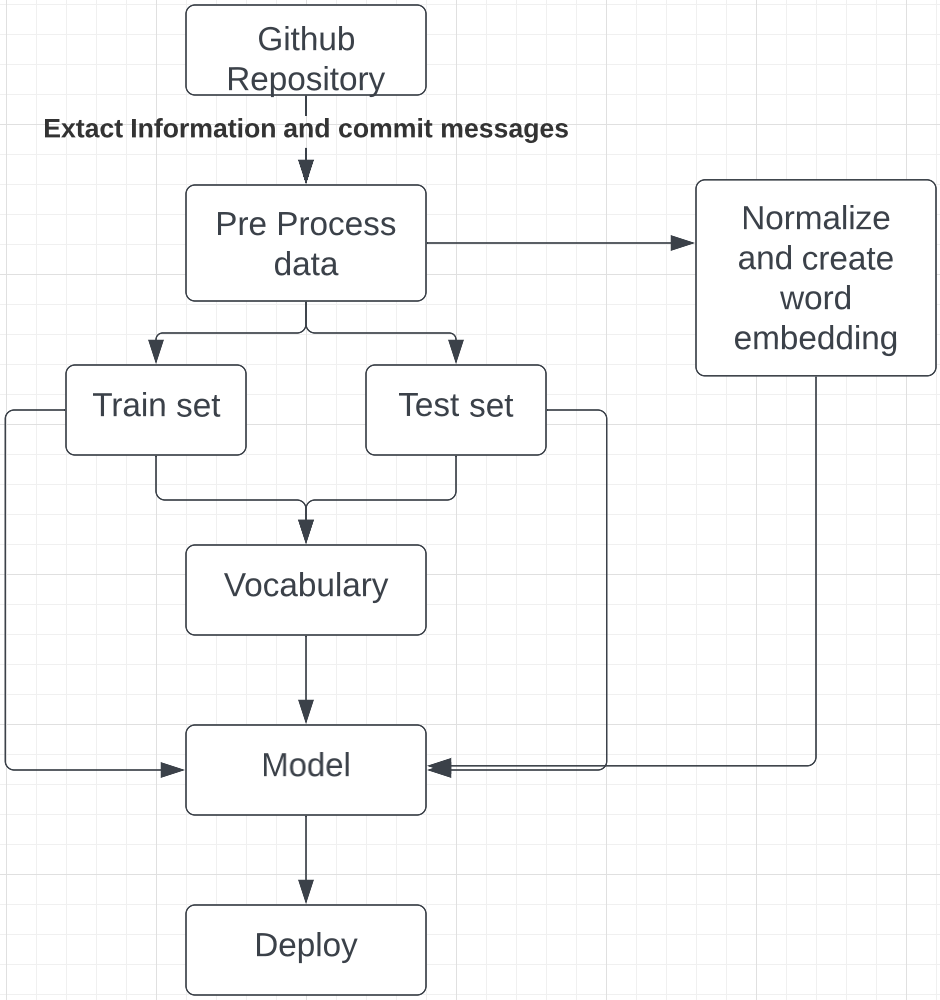
\includegraphics[width=5cm]{Flowchart.png}
     \caption{Flowchart}
     \label{fig:my_label}
 \end{figure}
 
\section{Experimental Results}
\label{Section: Result} 

The authors considered seven classifiers in their study. In our experiment, we considered those seven classifiers along with five other classifiers Xgboost, NN, Stack, Bagging, and Voting. We observed that the stack performs similarly to the decision tree in the first scenario. The accuracies range from 79\% to 83\% with xgboost being the worst performer among the five. In the inter-project scenario, the stack classifier performed better than the previously reported classifier. In the intra-project scenario, nn and xgboost performed better than LR with an accuracy of 77\%.

 \textbf{ RQ1 – How accurately can we predict test flakiness based on test smells in the test cases?}
\\
By first training and then evaluating the classifiers, the prediction model was developed. Every classifier had a reasonable performance archive except the Naive Bayes classifier with an accuracy of 65\%. Random Forest classifier had higher accuracy and precision of 83.6\%.
The collected results demonstrate that test smell-based models, with precision values ranging from 75\% to 83\%, perform reasonably well in predicting test flakiness. The trained classifiers were tested using the flaky tests included in the idFlakies dataset to confirm the model’s performance in the cross-project environment. The newly added classifiers performed similarly to the existing ones with accuracy ranging from 79\% to 83\%.


\begin{figure}
    \centering
    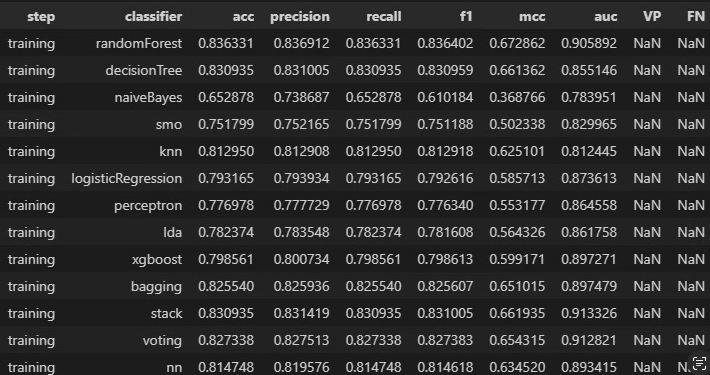
\includegraphics[width=7cm]{TrainingTestSmell.png}
    \caption{Training result parameters}
    \label{fig:my_label}
\end{figure}

In the intra-project scenario, the performance of all the classifiers is dropped. In a previous study, Logistic regression attained the highest score accurately identifying 26 out of 9 flaky tests. The newly added xgboost and nn classifiers had an accuracy of 77\% better than any other classifier.  In an inter-project scenario, the classifier’s performance declined more sharply. With recall values ranging from 48\% to 55\%, the classifiers do not differ significantly from one another, with Naive-Bayes reaching a value of 14\% by accurately identifying 17 out of 103 flaky tests. In the extended study, we found that the stack classifier has a recall of 56.6\%.
The results collected demonstrate that the smells can be utilized to predict flakiness. But, in the inter-project scenario, performance suffers significantly. The findings demonstrate that the performance of the smell-based models is equivalent to, and occasionally even superior to vocabulary model. The classifier’s performance ranges from 11\% to 56\%.
This led to the conclusion that smells are reliable indicators of flakiness.
\\
\begin{figure}
    \centering
    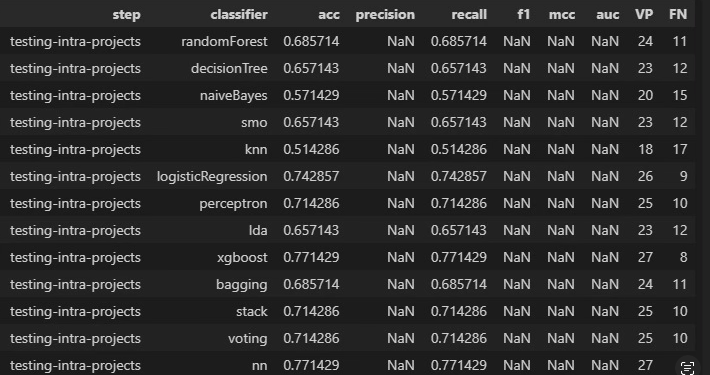
\includegraphics[width=7cm]{IntraProjects.png}
    \caption{Intra-Project}
    \label{fig:my_label}
\end{figure}

\begin{figure}
    \centering
    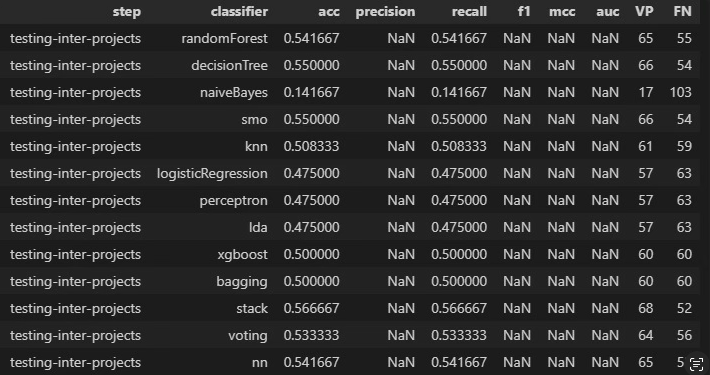
\includegraphics[width=7cm]{InterProjects.png}
    \caption{Inter-Project}
    \label{fig:my_label}
\end{figure}





\textbf{ RQ2 – Which attributes are the most strongly associated with test flakiness prediction?}

To identify associations between attributes and flakiness, we used sklearn.feature\textunderscore selection.mutual\textunderscore info\textunderscore classify method of scikit-learn that allows us to select features and in the future experiment by eliminating the least relevant features to optimize the model. The function calculates Mutual Information, which is the measure of the mutual dependence between two random variables. We use MI over Correlation between each attribute as it is more versatile and can capture non-linear relationships, while correlation is limited to linear relationships. 
\\
\textbf{The equation for MI between a feature X and a target variable y is:}\\
\\\begin{math}MI(X, y) = \sum p(x,y) * log(p(x,y) / (p(x) * p(y)))\end{math}
\\
\\
While PCA Is a great Dimensionality tool, its usage as a feature selection is controversial due to the information loss it causes, as well as the reduced flexibility to manually select attributes to eliminate.
\begin{figure}
    \centering
    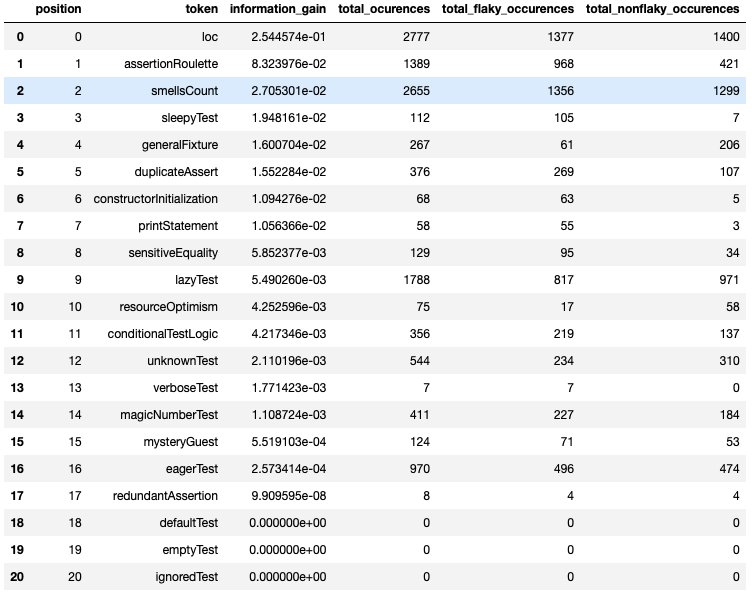
\includegraphics[width=7cm]{Tokens.png}
    \caption{Features}
    \label{fig:my_label}
\end{figure}
We identified that the most relevant feature in the dataset was loc (lines of Code) followed by assertion roulette (test smell), while the least relevant feature turned out to be redundant assertion (which is a test smell). Whereas, IgnoredTest, emptyTest, and defaultTest have no relation with an absolute zero score, thus indicating the need to drop the three columns.
The dataset only identifies if a test is flaky with a binary representation without the inclusion of any magnitude to provide the extent of flakiness, which might produce some limitations and could be scope for future experimentation.
\\
\begin{figure}
    \centering
    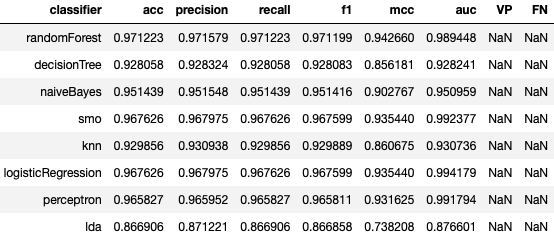
\includegraphics[width=7cm]{vocabulary apporach.png}
    \caption{Vocabulary-based approach}
    \label{fig:my_label}
\end{figure}

\textbf{ RQ3 – How does the test smell-based approach compare with the existing vocabulary-based approach?}
\\
 In the vocabulary-based approach, the values of VP (True Positive) and FN (False Negative) for the classification metrics are NaN (Not a Number). This is due to the dataset used for evaluation in the vocabulary-based approach only containing flaky tests and excluding non-flaky tests. As a result, this dataset lacks True Negatives (TN) and False Negatives (FN), making it impossible to calculate VP and FN.

Precision, recall, and F1-score for the vocabulary-based technique cannot be determined in the absence of TN and FN data. The accuracy and AUC numbers for this technique are the only ones that the authors have reported.
We trained the classifiers with the training and testing dataset using the vocabulary-based approach. The vocabulary-based strategy performs better than the smell-based approach: the best F1 score for vocabulary-based models is 97\% (Random Forest), while the score for the smell-based approach is 83\%. (Random Forest). The disparity is greater when MCC is analyzed. The best outcome for the smell-based technique was 0.66, and the best result for the vocabulary-based approach was 0.94. This score takes into consideration true and false positives, as well as negatives.
The cross-project validation results, however, demonstrate that the test smell-based strategy yields superior outcomes. The test smell-based strategy yielded 74\% of recall (LR) in the intra-project context, while the vocabulary-based approach only managed to reach 57\%. (KNN).



Using the training and testing datasets, the performance of the vocabulary-based models is superior to that of the test smell-based models. Yet, the smell-based approach achieves noticeably higher outcomes in the intra-project and inter-project contexts in the cross-project validation scenario.

\section{Example}
\label{section:Example}
Here we take the example of the Hadoop source code by running our model on it.
\\
\\
The following table shows the confusion matrix of our model on the data.\\
\\
\begin{center}
\begin{tabular}{|c|c|c|}
\hline
     & Positive & Negative \\
\hline
True & 1247 & 130 \\
\hline
False & 126 & 1274 \\
\hline
\end{tabular}
\end{center}

The attributes are generated by TsDetect and here we show the cases of each of the conditions where the model fails and succeeds. We also show the confusion matrix when running on the validation set. Figure 8 shows the test case isOriginalTGTReturnsCorrectValues() belongs to the TestSecurityUtil class of the Hadoop source code. Figures 9 show the case where the model fairly recognized it as a flaky test while it wasn't one belonging to the False Positive part of the population. Figures 10 and 13 show the cases where our model was successfully able to identify if the tests were flaky. Figure 12 shows the case where our model identified the test as flaky successfully.


\begin{figure}
    \centering
    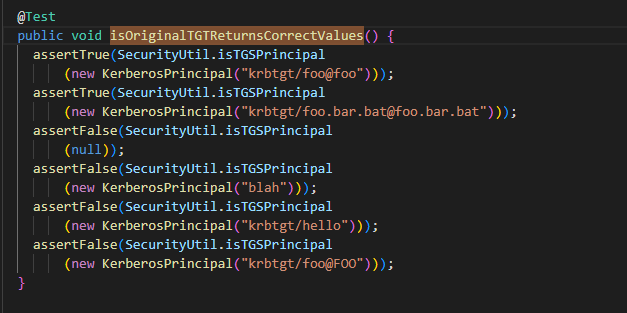
\includegraphics[scale=0.4]{ConfusionMatrix/fntest.png}
    \caption{False Negative TestCase}
    \label{fig:my_label}
\end{figure}

\begin{figure}
    \centering
    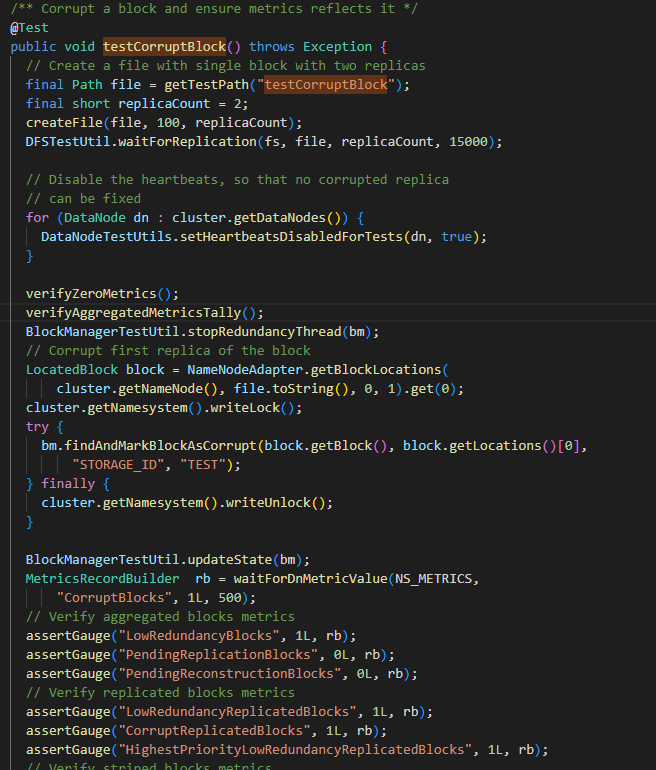
\includegraphics[scale=0.3]{ConfusionMatrix/fptest.png}
    \caption{False Positive TestCase}
    \label{fig:my_label}
\end{figure}

\begin{figure}
    \centering
    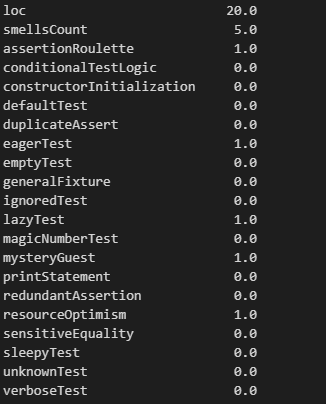
\includegraphics[scale=0.5]{ConfusionMatrix/tnpara.png}
    \caption{True negative Parameters}
    \label{fig:my_label}
\end{figure}

\begin{figure}
    \centering
    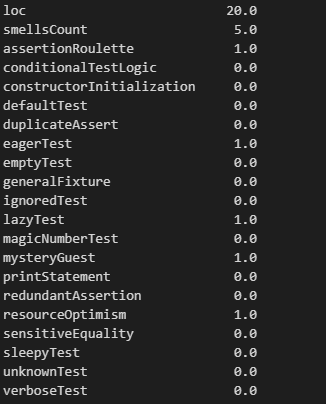
\includegraphics[scale=0.3]{ConfusionMatrix/tnpara.png}
    \caption{True negative TestCase}
    \label{fig:my_label}
\end{figure}

\begin{figure}
    \centering
    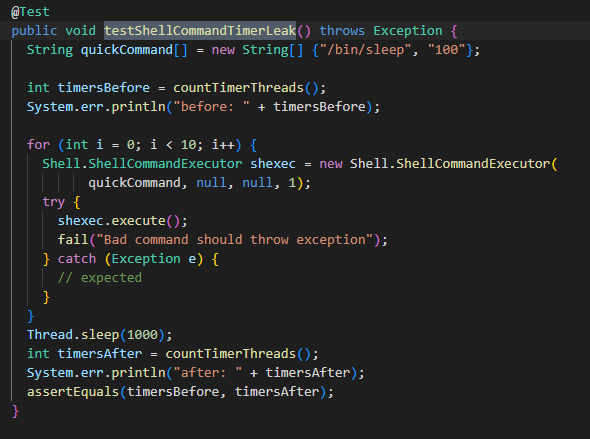
\includegraphics[scale=0.3]{ConfusionMatrix/tptest.png}
    \caption{True positive TestCase}
    \label{fig:my_label}
\end{figure}


\begin{figure}
    \centering
    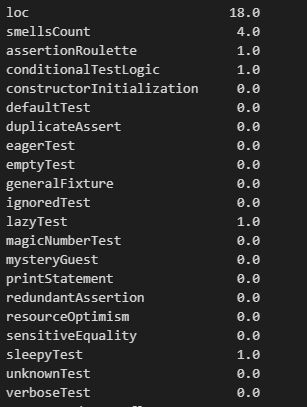
\includegraphics[scale=0.3]{ConfusionMatrix/tppara.png}
    \caption{True Positive Parameters}
    \label{fig:my_label}
\end{figure}


 \section{Discussion}
 \label{Section:Discussion}
 The findings of our study show that using test smells to predict flaky tests can be useful. All of the investigated classifiers (Random Forest, Decision Tree, Logistic Regression, KNN, XGBoost, Bagging, Stack, NN, and Voting) achieved a fair level of accuracy in identifying flaky tests, according to our research. The Random forest classifier performed the best, followed closely by the decision tree, bagging, and stack  classifiers, with Voting and KNN coming third and fourth. The naive Bayes classifier performs the worst with an accuracy of just 65\%. Furthermore, our findings indicate that the use of test smells is particularly effective in predicting flaky tests for projects in the same domain. In the inter-project scenario, the stack performs better than previously reported logistic regression with an accuracy of 56\%. In the intra-project scenario, Xgboost and NN perform better than LR with an accuracy of 77\% Intra-project testing was substantially more accurate than inter-project testing, implying that using test smells within a project rather than across various projects may be more helpful in identifying flaky tests. This finding is consistent with prior research that found flakiness to be more prevalent within a project rather than across multiple projects.
 \\
\subsection{Implications for Practitioners:}
\label{subsection:1}
The findings of this study show that among the five additional classifiers stack predict test smells identical to the Decision tree classifier and very close to the best-performing classifier Random forest. As a result, practitioners should think about incorporating any of these classifiers into their test smell prediction tasks. An implication of this study is that when predicting test smells, practitioners should not rely entirely on a single classifier. They could instead explore utilizing numerous classifiers and comparing their predictions to achieve improved accuracy and resilience. The study's findings are valuable for practitioners involved in software testing and quality assurance. Practitioners can increase the accuracy and reliability of their test smell prediction jobs by combining multiple classifiers and exploiting their particular strengths, which can lead to more efficient and successful software development processes.
 \\
\subsection{Implications for Researchers:}
\label{subsection:2}
The newly included classifiers, XGBoost, Bagging, Stacking, NN, and Voting, did not outperform the best classifier, Random Forest. This shows that adding more complicated classifiers may not result in a meaningful improvement in the performance of test smell prediction models. As a result, more work could be invested in creating more effective feature selection strategies while also investigating other areas of prediction models such as hyperparameter tuning and ensemble techniques. Additionally, researchers could look into combining different classifiers with the random forest to potentially improve the model's performance. Furthermore, future research could look into the use of deep learning techniques to predict test smells.

\\
\subsection{Implications for Tool builders:}
\label{subsection:3}
The results of this study imply that tool builders should think about testing their tools with several classifiers. Using different classifiers provides for a more thorough examination of the tool's usefulness and can provide additional insights into the tool's performance. Furthermore, tool builders should consider the trade-off between classifier performance and the computational resources required to run them. They should continue to investigate new machine-learning techniques and algorithms. While the new classifiers evaluated in this study performed similarly to the Random Forest, other algorithms may outperform it and provide more accurate test smell predictions. As a result, tool developers must stay up to date on breakthroughs in the field of machine learning and evaluate new techniques as they become available. 
 \section{Threats To Validity}
 \label{Section:Threats}

\textbf{Construct Validity:}
 The degree to which a concept is operationalized (i.e., how it is measured) accurately reflects the intended construct is known as its construct validity. The relation between test smells and the flaky test is the construct that interests this study's researchers. To operationalize this concept,  a variety of test smells, including the assertion roulette and conditional test logic were considered. There is a potential threat to the identification of the flaky tests.\\
 The most widely used metrics in the machine learning (ML) community were adopted to evaluate the classifiers in order to reduce this threat, which can aid in improving the study's generalizability and reliability. However, the authors utilized a program called tsDetect to find test smells in the code during the pre-processing stage of the test code. The production class, a vital component of the codebase that the tests are testing, has occasionally been missed by tsDetect. As a result, there were instances where test smells could not be extracted from the code, which could jeopardize the study's findings.
\\

\textbf{Internal Validity:}
 The degree to which a research study accurately ascertains the link between the independent variable and the dependent variable is referred to as internal validity. The existence of confounding variables, which are variables that can impact the relationship between the independent and dependent variables, is one factor that could endanger internal validity. Confounding variables in this study may include things like the size and complexity of the codebase, the level of experience of the developers, and the particular programming language employed. The authors employed statistical techniques like logistic regression and decision trees to account for the effects of these confounding variables and identify the association between test smells and flaky tests in order to address this possible danger.
\\

 \textbf{External Validity:}
 The generalizability of research findings may be constrained by factors that pose a threat to external validity. Four open-source projects were utilized by the authors to gather data for their study, although other software projects in different domains or with various characteristics might not be comparable to these projects. The results may not apply to projects created in other programming languages, for instance, since all of the projects utilized in the study were written in Java. The study's projects were small to medium-sized, and the authors also pointed out that they might not accurately represent the features of larger software projects because of their size. The authors emphasized the limits of their study and suggested that future research should investigate whether or not their findings apply to other software projects and domains in order to address this possible threat.
\\

\textbf{Conclusion Validity:}
The degree to which the inferences made from the data accurately reflect the underlying relationships between the variables under investigation is referred to as conclusion validity.
The authors of the research thoroughly analyzed their data and assessed how well their classifier models performed using the relevant statistical methods. They also talked about some of the study's possible drawbacks, namely the use of a single dataset and the scant number of projects examined. They did not, however, point out any particular problems or worries regarding the inferences made from the data.




 \section{Future Work}
 \label{Section:FutureWork}
 A promising solution to the problem of finding and anticipating flaky tests in software testing is presented by the authors. More study in this area is still needed. The current study focused on a particular set of test smells, but there might be additional clues that might be used to spot and foretell problematic testing. To increase the accuracy of shaky test prediction models, future studies could include other test smells or other elements, such as code complexity or ambient elements. Despite the study's encouraging predictions for flaky tests, it is crucial to comprehend how employing test smells impacts the entire software testing process. Future studies could look into how using test smells affects testing effectiveness, efficiency, and overall software product quality. The tsDetect tool was used in the investigation to find test smells in the codebase. Nonetheless, this tool's accuracy and dependability could yet be enhanced. Future studies could concentrate on creating more advanced tools or enhancing currently available technologies more correctly and effectively detect test scents. The study does not address the fundamental reasons for flakiness, even if it offers a means to recognize and anticipate flaky tests. Future studies could look at the underlying factors that contribute to flaky testing and devise methods to stop them from happening in the first place.


 \section{Conclusion}
 \label{Section:Conclusion}
According to the study, a number of test smells, such as assertion roulette and conditional test logic, were strongly linked to flaky tests. Based on these smells, the classifiers created using machine learning approaches were highly accurate in predicting flaky tests.
The accuracy of the test smell detection tool and the small size and scope of the dataset utilized in the study are two major risks to the validity of the study, the authors point out. The authors contend that additional study is required to both explore additional variables that can affect test flakiness in software testing and to confirm the efficacy of test smells as predictors of flaky tests.
Overall, the study offers insightful information about the use of test smells as a viable method for enhancing the accuracy and effectiveness of software testing.
 
 \bibliographystyle{ACM-Reference-Format}
 \bibliography{citations}


% \setcounter{page}{1}        % set page counter
% \pagenumbering{arabic}      % set page number style
% \pagestyle{fancy}         % top right page numbers
% %\pagestyle{cornell}
% %\pagestyle{cornellc}       % centered page numbers, disables drafthead

% % \renewcommand{\chaptermark}[1]{\markboth{#1}{}}
% % \renewcommand{\sectionmark}[1]{\markright{#1}{}}

% \fancyhead{} % clear all fields


\end{document}

\endinput
%%
%% End of file `sample-authordraft.tex'.
